% Regression slice derived from PGF manual section "Shapes with Multiple Parts".
% It exercises the real empty-part height/depth keys rather than a case-specific layout.
\documentclass[tikz,border=2pt]{standalone}
\usetikzlibrary{shapes.multipart}
\begin{document}
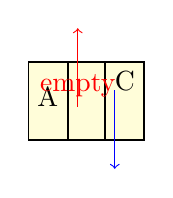
\begin{tikzpicture}
  \node[
    rectangle split,
    rectangle split horizontal,
    rectangle split parts=3,
    rectangle split empty part width=2pt,
    rectangle split empty part height=3ex,
    rectangle split empty part depth=2ex,
    rectangle split part align={base,center,top},
    draw,
    fill=yellow!15
  ] (parts) {A\nodepart{two}\nodepart{three}C};

  \draw[red,->] (parts.two) -- ++(0,1cm);
  \draw[blue,->] (parts.three) -- ++(0,-1cm);
  \node[above,red] at (parts.two) {empty};
\end{tikzpicture}
\end{document}
